\documentclass[12pt,a4paper]{article}
\usepackage[top=2.2cm,bottom=2.2cm,left=2.2cm,right=2.2cm]{geometry}
\usepackage{newtxtext,newtxmath}
\usepackage{booktabs,longtable,array,xcolor,graphicx}
\usepackage[hidelinks]{hyperref}
\usepackage{titlesec}
\titleformat{\section}{\large\bfseries}{}{0pt}{}
\titlespacing*{\section}{0pt}{14pt}{6pt}
\newcolumntype{P}[1]{>{\raggedright\arraybackslash}p{#1}}
\setlength{\LTleft}{0pt}\setlength{\LTright}{0pt}
\setlength{\tabcolsep}{5pt}
\renewcommand{\arraystretch}{1.15}
\setlength{\parskip}{5pt}
\setlength{\parindent}{0pt}
\pagestyle{plain}

\begin{document}

\begin{center}
{\Large\bfseries Response to Reviewers' Comments}\\[4pt]
Paper ID 2147 \quad\textbullet\quad ICMLDE 5.0 \quad\textbullet\quad Procedia Computer Science
\end{center}

\begin{tabular}{@{}lp{0.78\textwidth}@{}}
\textbf{Original title:} & \emph{Edge-Deployable Skin Lesion Classification: A Weighted Ensemble of MobileNetV2 and DINOv2}\\
\textbf{Revised title:} & \emph{Edge-Deployable Skin Lesion Classification with Quantized CNN and Transformer Models}
\end{tabular}

\medskip
Respected Scientific Committee and Reviewers,

We sincerely thank the reviewers for their careful reading and constructive comments, which have substantially strengthened the paper. In addressing them, we carried out a detailed audit of the data split and of the model-fusion evaluation, which sharpened the focus of the contribution. The revised paper presents MobileNetV2 and DINOv2 as independent branches, analyses their probability-level fusion with a paired statistical test, and adds on-device latency, memory, and thermal measurements on a Raspberry Pi 4 for the FP32 and quantized models. All accuracies are reported transparently as validation results, together with a lesion-level overlap analysis.

\section*{Summary of Major Changes}
\begin{enumerate}
\item \textbf{Title:} revised from ``Edge-Deployable Skin Lesion Classification: A Weighted Ensemble of MobileNetV2 and DINOv2'' to ``Edge-Deployable Skin Lesion Classification with Quantized CNN and Transformer Models''.
\item \textbf{Block diagram (Fig.~1):} redrawn to show data preparation, the two independent MobileNetV2 and DINOv2 branches with their baseline FP32 evaluation and optimization experiments, Grad-CAM explainability, the three output classes, and the Raspberry Pi 4 deployment with its measured latency.
\item \textbf{Methodology:} the two models are presented as independent branches, and probability-level fusion is analysed in a dedicated section with a paired McNemar test (Sec.~3.6 and 4.4).
\item \textbf{Edge deployment:} new Section~4.6 and Table~4 report Raspberry Pi 4 latency, throughput, peak memory, and sustained thermal behaviour for the FP32 and quantized models.
\item \textbf{Data analysis:} lesion-level overlap audit (Sec.~3.2), justification of the three classes, and class-balance statistics (Sec.~3.1).
\item \textbf{Results and figures:} training curves redrawn as one four-panel figure (Fig.~3), MobileNetV2 confusion matrix and per-class table (Fig.~4, Table~5), and a new Grad-CAM section with Fig.~5.
\item \textbf{Text:} abstract, introduction, contributions, discussion, and conclusion rewritten to reflect these changes.
\item \textbf{References:} seven references added, four previously uncited references now cited, and the list numbered in order of citation.
\end{enumerate}

\begin{center}
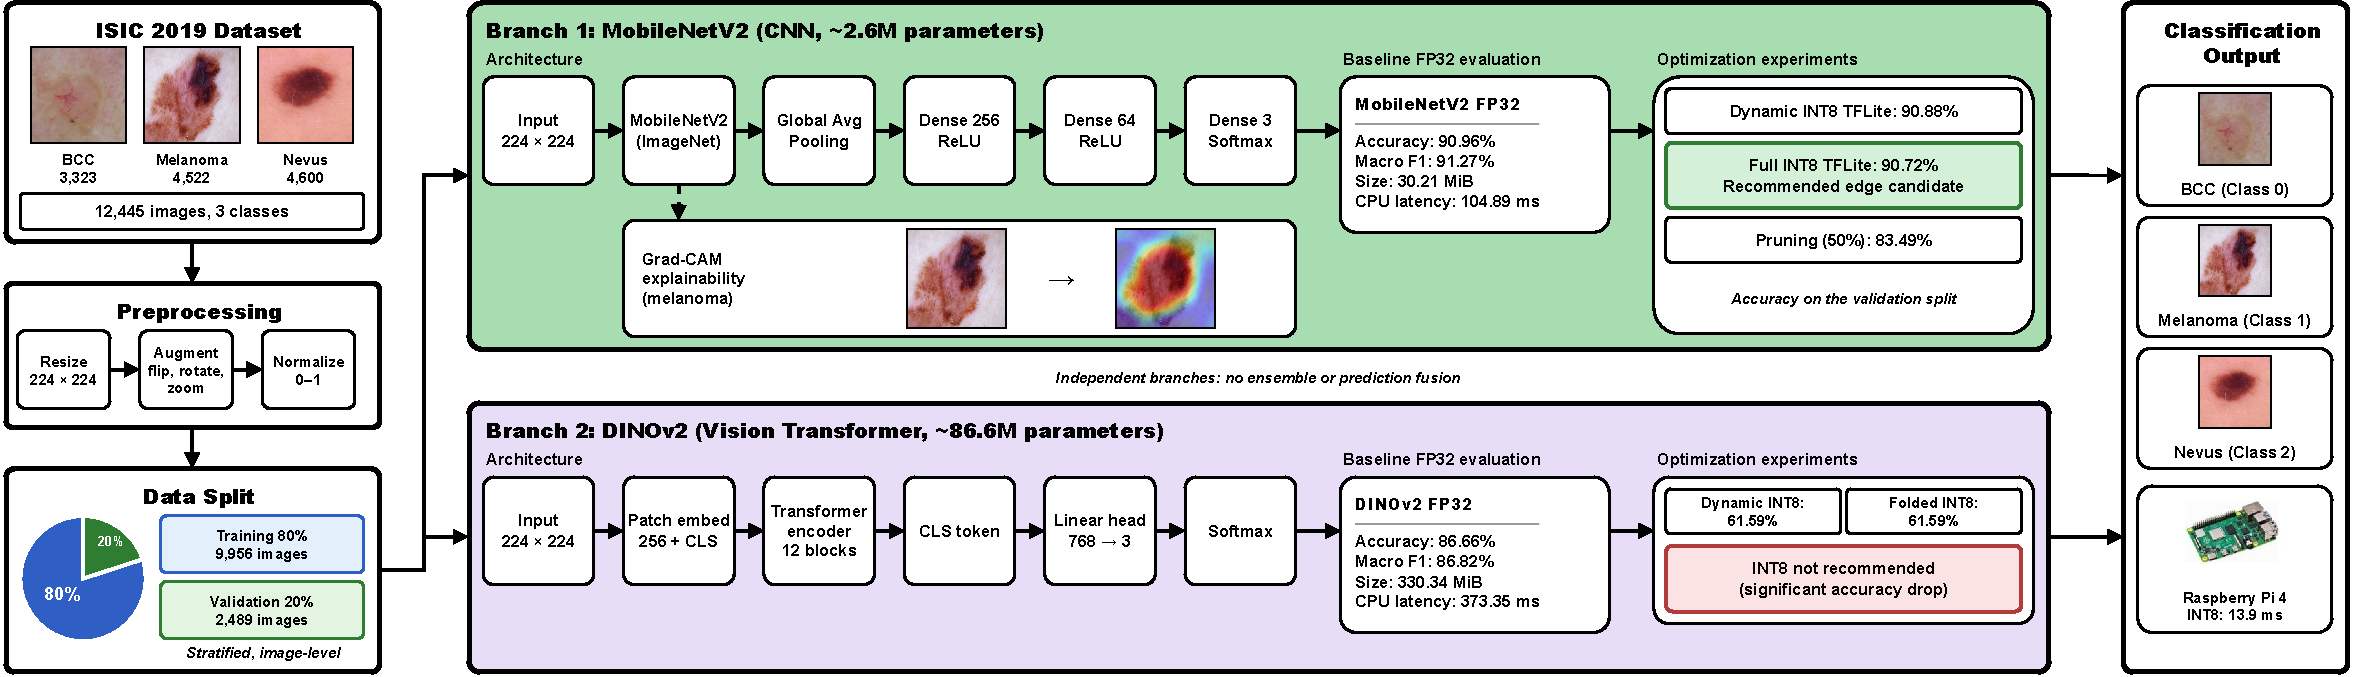
\includegraphics[width=\textwidth]{dermavision_architecture.pdf}\\[4pt]
\small\textbf{Revised block diagram (Fig.~1 of the revised manuscript).}
\end{center}

\section*{Point-by-Point Responses}
Page numbers below refer to the revised manuscript.

\section*{Reviewer 1}
\textbf{Comment 1.1:} \emph{The abstract reports validation accuracy; independent test results should be reported.}

\textbf{Response:} We thank the reviewer for this important observation. The abstract and all results now state explicitly that they are validation results, together with the reason: a lesion-ID audit found 54.04\% overlap between validation and training lesions. We also report accuracy on the 1,144 validation images whose lesions do not appear in training (MobileNetV2 86.80\%, DINOv2 84.00\%), which is the closest available unbiased estimate. A lesion-grouped split with no lesion overlap has been prepared, and retraining with a single held-out test evaluation on it is listed as the first item of future work.

\begin{center}
\begin{minipage}{\linewidth}\centering
\small
\textbf{Accuracy on the full and the non-overlapping validation images}\\[3pt]
\begin{tabular}{lcc}
\toprule
\textbf{Model} & \textbf{All 2,489 images} & \textbf{1,144 non-overlapping images} \\
\midrule
MobileNetV2 FP32 & 90.96\% & 86.80\% \\
DINOv2 FP32 & 86.66\% & 84.00\% \\
Equal-weight fusion & 91.36\% & 87.15\% \\
\bottomrule
\end{tabular}
\end{minipage}
\end{center}

\textbf{Revised in the manuscript} (Abstract (p.~1); Sec.~3.2 (p.~4)): ``\ldots\ \emph{All results are validation results, because lesion-level auditing identified 54.04\% overlap between validation and training images.} \ldots''

\vspace{10pt}\noindent\rule{\textwidth}{0.4pt}\vspace{4pt}
\textbf{Comment 1.2:} \emph{A weighted ensemble of MobileNetV2 and DINOv2 is a modest contribution.}

\textbf{Response:} We thank the reviewer for this valuable comment. In response, the contribution has been redefined around edge deployment: the revised paper presents (i) a controlled comparison of FP32, dynamic-range INT8, full-integer INT8, and 50\% pruned MobileNetV2; (ii) on-device latency, memory, and thermal measurements on a Raspberry Pi 4; and (iii) an analysis of INT8 quantization for DINOv2, including the activation outliers in Blocks 8--11. The probability-level fusion is retained as a supporting analysis, and the title now reflects quantization as the central subject.

\textbf{Revised in the manuscript} (Title; Abstract (p.~1); Sec.~3.6 (p.~4); Sec.~4.4 (p.~6)): ``\ldots\ \emph{The two models are evaluated as independent branches; a post-hoc probability-fusion audit gave no reliable gain over MobileNetV2, so fusion is not part of the pipeline.} \ldots''

\vspace{10pt}\noindent\rule{\textwidth}{0.4pt}\vspace{4pt}
\textbf{Comment 1.3:} \emph{The edge-deployable claim needs latency and memory measurements on edge devices.}

\textbf{Response:} We thank the reviewer for this suggestion. All MobileNetV2 variants were benchmarked on a Raspberry Pi 4 Model B (4 GB, Cortex-A72, CPU only). Full INT8 TFLite ran at 13.92~ms per image (71.8 FPS) with 51.7~MiB peak memory, compared with 597.59~ms and 636.9~MiB for the FP32 Keras model; an unquantized FP32 TFLite baseline (36.63~ms) separates the runtime effect from the quantization effect. Sustained 5-minute runs reached at most 78.4\,$^\circ$C with no throttling, and the Full INT8 latency remained constant (14.11 to 14.16~ms).

\begin{center}
\begin{minipage}{\linewidth}\centering
\small
\textbf{Raspberry Pi 4 Model B results (batch one, four threads)}\\[3pt]
\begin{tabular}{lccccc}
\toprule
\textbf{Variant} & \textbf{Disk} & \textbf{Latency (ms)} & \textbf{FPS} & \textbf{Peak RSS} & \textbf{Max temp.} \\
\midrule
FP32 Keras & 30.21 MiB & 597.59 $\pm$ 9.86 & 1.67 & 636.9 MiB & 55.0\,$^\circ$C \\
FP32 TFLite & 9.79 MiB & 36.63 $\pm$ 0.34 & 27.30 & 69.5 MiB & 74.5\,$^\circ$C \\
Dynamic-range INT8 & 2.74 MiB & 41.72 $\pm$ 3.42 & 23.97 & 59.2 MiB & 72.0\,$^\circ$C \\
\textbf{Full INT8} & \textbf{2.94 MiB} & \textbf{13.92 $\pm$ 0.20} & \textbf{71.83} & \textbf{51.7 MiB} & \textbf{78.4\,$^\circ$C} \\
\bottomrule
\end{tabular}
\end{minipage}
\end{center}

\textbf{Revised in the manuscript} (Sec.~4.6, Table~4 (p.~7)): ``\ldots\ \emph{Full INT8 TFLite ran at 13.92 ms per image (71.8 FPS), 42.9$\times$ faster than FP32 Keras and 2.6$\times$ faster than unquantized FP32 TFLite, while using the least memory.} \ldots''

\vspace{10pt}\noindent\rule{\textwidth}{0.4pt}\vspace{4pt}
\textbf{Comment 1.4:} \emph{Ensemble weights tuned on validation data must be tested on a separate test set.}

\textbf{Response:} We thank the reviewer for this point. As a separate test set was not available, weighted fusion was kept out of the deployed pipeline rather than reporting a tuned result as test performance. Section~4.4 reports both evaluated weightings against MobileNetV2 alone and notes the selection effect of choosing weights on the validation predictions.

\textbf{Revised in the manuscript} (Sec.~3.6 (p.~4)): ``\ldots\ \emph{This fusion is an audit only and is not part of the DermaVision pipeline shown in Figure~1.} \ldots''

\vspace{10pt}\noindent\rule{\textwidth}{0.4pt}\vspace{4pt}
\textbf{Comment 1.5:} \emph{Comparison with published ISIC 2019 results is needed.}

\textbf{Response:} We thank the reviewer for this suggestion. Published ISIC 2019 results are reported on the full eight-class task, mostly with balanced accuracy, and on splits that are rarely lesion-disjoint, whereas this study uses a three-class subset and an image-level split with documented lesion overlap. A side-by-side accuracy table would therefore compare different tasks. The revised manuscript instead states the task scope explicitly and focuses on a controlled comparison of model and compression variants under one protocol, where every number is directly comparable.

\textbf{Revised in the manuscript} (Abstract (p.~1); Sec.~5 (p.~8--9)): ``\ldots\ \emph{The results therefore support comparative compression and deployment analysis, but not clinical generalization.} \ldots''

\vspace{10pt}\noindent\rule{\textwidth}{0.4pt}\vspace{4pt}
\textbf{Comment 1.6:} \emph{The conclusion should discuss the small 1.24-point gain.}

\textbf{Response:} We thank the reviewer for this comment. Based on the verified predictions, the equal-weight fusion improves on MobileNetV2 by 0.40 points (10 additional correct images; McNemar $p = 0.174$), while the 0.4/0.6 configuration gave 90.76\%. The Discussion and Conclusion now discuss this modest gain and explain why the Full INT8 MobileNetV2 is selected as the deployment model.

\begin{center}
\begin{minipage}{\linewidth}\centering
\small
\textbf{Fusion analysis on the 2,489 validation images}\\[3pt]
\begin{tabular}{lccc}
\toprule
\textbf{Configuration} & \textbf{Accuracy} & \textbf{Macro F1} & \textbf{Melanoma recall} \\
\midrule
MobileNetV2 FP32 & 90.96\% & 91.27\% & 87.06\% \\
DINOv2 FP32 & 86.66\% & 86.82\% & 79.09\% \\
Fusion ($w_M=0.5$, $w_D=0.5$) & 91.36\% & 91.67\% & 87.39\% \\
Fusion ($w_M=0.4$, $w_D=0.6$) & 90.76\% & 91.01\% & 85.18\% \\
\bottomrule
\end{tabular}
\end{minipage}
\end{center}

\textbf{Revised in the manuscript} (Sec.~4.4 (p.~6)): ``\ldots\ \emph{An exact two-sided McNemar test on these discordant pairs gave $p = 0.174$, so the improvement is not statistically significant at the 0.05 level; the test also assumes independent samples, which the documented lesion overlap only partly satisfies.} \ldots''


\section*{Reviewer 2}
\textbf{Comment 2.1:} \emph{Only three classes are used; the selection should be justified.}

\textbf{Response:} We thank the reviewer for this suggestion. The three classes were chosen because they cover a malignant melanocytic lesion (Melanoma), its most common benign look-alike (Nevus), and the most common non-melanocytic skin cancer (BCC). This isolates the clinically most consequential Melanoma--Nevus confusion and keeps the class distribution comparatively balanced. The limitations of this choice are stated in the Discussion.

\textbf{Revised in the manuscript} (Sec.~3.1 (p.~3)): ``\ldots\ \emph{They cover a malignant melanocytic lesion, its most common benign look-alike, and the most common non-melanocytic skin cancer, which isolates the clinically most consequential Melanoma--Nevus confusion.} \ldots''

\vspace{10pt}\noindent\rule{\textwidth}{0.4pt}\vspace{4pt}
\textbf{Comment 2.2:} \emph{Per-class recall, especially for melanoma, should be reported.}

\textbf{Response:} We thank the reviewer for this suggestion. Table~5 reports per-class precision, recall, and F1 for MobileNetV2 (Melanoma recall 87.06\%), Table~3 reports Melanoma recall for every model variant, and the confusion matrix in Fig.~4 shows that the main error is Melanoma predicted as Nevus (78 images).

\begin{center}
\begin{minipage}{\linewidth}\centering
\small
\textbf{Class-level performance of MobileNetV2 FP32}\\[3pt]
\begin{tabular}{lcccc}
\toprule
\textbf{Class} & \textbf{Support} & \textbf{Precision} & \textbf{Recall} & \textbf{F1-score} \\
\midrule
BCC & 665 & 93.04\% & 96.54\% & 94.76\% \\
Melanoma & 904 & 89.03\% & 87.06\% & 88.03\% \\
Nevus & 920 & 91.26\% & 90.76\% & 91.01\% \\
Macro average & 2,489 & 91.11\% & 91.45\% & 91.27\% \\
\bottomrule
\end{tabular}
\end{minipage}
\end{center}

\textbf{Revised in the manuscript} (Sec.~4.7, Fig.~4, Table~5 (p.~8)): ``\ldots\ \emph{BCC achieved the highest recall, while Melanoma achieved the lowest.} \ldots''

\vspace{10pt}\noindent\rule{\textwidth}{0.4pt}\vspace{4pt}
\textbf{Comment 2.3:} \emph{Class balance should be described.}

\textbf{Response:} We thank the reviewer for this suggestion. The dataset contains 3,323 BCC, 4,522 Melanoma, and 4,600 Nevus images; the stratified split gives 2,658 / 3,618 / 3,680 training and 665 / 904 / 920 validation images. The classes are therefore close to balanced (largest-to-smallest ratio 1.38), and the stratified split preserves these proportions in both partitions.

\begin{center}
\begin{minipage}{\linewidth}\centering
\small
\textbf{Class distribution}\\[3pt]
\begin{tabular}{lccc}
\toprule
\textbf{Class} & \textbf{Total} & \textbf{Training (80\%)} & \textbf{Validation (20\%)} \\
\midrule
BCC & 3,323 & 2,658 & 665 \\
Melanoma & 4,522 & 3,618 & 904 \\
Nevus & 4,600 & 3,680 & 920 \\
\textbf{Total} & \textbf{12,445} & \textbf{9,956} & \textbf{2,489} \\
\bottomrule
\end{tabular}
\end{minipage}
\end{center}

\textbf{Revised in the manuscript} (Sec.~3.1 (p.~3)): ``\ldots\ \emph{The subset contains 3,323 BCC, 4,522 Melanoma, and 4,600 Nevus images (largest-to-smallest ratio 1.38), so the classes are close to balanced.} \ldots''

\vspace{10pt}\noindent\rule{\textwidth}{0.4pt}\vspace{4pt}
\textbf{Comment 2.4:} \emph{Lesion-level splitting should be confirmed.}

\textbf{Response:} We thank the reviewer for this important point. A lesion-ID audit was carried out and is now reported in Section~3.2: the split is image-level, and 54.04\% of validation images belong to lesions present in training (BCC 85.11\%, Melanoma 79.31\%, Nevus 6.74\%). The manuscript reports this transparently, gives results on the non-overlapping subset, and a lesion-grouped split has been prepared for retraining in future work.

\begin{center}
\begin{minipage}{\linewidth}\centering
\small
\textbf{Share of validation images whose lesion also appears in training}\\[3pt]
\begin{tabular}{lc}
\toprule
\textbf{Class} & \textbf{Validation images with lesion overlap} \\
\midrule
BCC & 85.11\% \\
Melanoma & 79.31\% \\
Nevus & 6.74\% \\
\textbf{All classes} & \textbf{54.04\%} \\
\bottomrule
\end{tabular}
\end{minipage}
\end{center}

\textbf{Revised in the manuscript} (Sec.~3.2 (p.~4)): ``\ldots\ \emph{Of the validation images, 1,345 (54.04\%) belonged to lesions also represented in the training partition.} \ldots''

\vspace{10pt}\noindent\rule{\textwidth}{0.4pt}\vspace{4pt}
\textbf{Comment 2.5:} \emph{Statistical significance should be tested.}

\textbf{Response:} We thank the reviewer for this suggestion. An exact two-sided McNemar test compares MobileNetV2 with the equal-weight fusion on the same 2,489 images: the fusion corrected 27 MobileNetV2 errors and introduced 17 new ones ($p = 0.174$), so the 0.40-point gain is not statistically significant at the 0.05 level. The manuscript reports this result and lists confidence intervals on a lesion-disjoint test set as future work.

\begin{center}
\begin{minipage}{\linewidth}\centering
\small
\textbf{Paired outcomes of MobileNetV2 and the equal-weight fusion (McNemar)}\\[3pt]
\begin{tabular}{lcc}
\toprule
\textbf{} & \textbf{Fusion correct} & \textbf{Fusion wrong} \\
\midrule
MobileNetV2 correct & 2,247 & 17 \\
MobileNetV2 wrong & 27 & 198 \\
\bottomrule
\end{tabular}
\end{minipage}
\end{center}
\begin{center}\small Exact two-sided McNemar test on the discordant pairs (27 vs.\ 17): $p = 0.174$.\end{center}

\textbf{Revised in the manuscript} (Sec.~4.4 (p.~6)): ``\ldots\ \emph{Equal-weight fusion corrected 27 MobileNetV2 errors and introduced 17 new ones, a net gain of 10 images, and raised recall in every class (BCC $+0.30$, Melanoma $+0.33$, Nevus $+0.54$ percentage points).} \ldots''

\vspace{10pt}\noindent\rule{\textwidth}{0.4pt}\vspace{4pt}
\textbf{Comment 2.6:} \emph{Limitations of using a three-class subset of ISIC 2019 should be stated.}

\textbf{Response:} We thank the reviewer for this suggestion. The Discussion now states that only three of the eight ISIC 2019 categories are used, that 1,886 images lack lesion IDs, and that external multi-centre validation is not yet included, so the results are presented as comparative rather than clinical evidence.

\textbf{Revised in the manuscript} (Sec.~5 (p.~8--9)): ``\ldots\ \emph{The dataset also contains only three of the eight ISIC 2019 categories, includes 1,886 images without lesion IDs, and has no external multi-centre validation.} \ldots''


\section*{Reviewer 3}
\textbf{Comment 3.1:} \emph{DINOv2 deployment on edge devices should be discussed.}

\textbf{Response:} We thank the reviewer for this suggestion. DINOv2 FP32 requires 330.34~MiB and 235--373~ms per image on the development CPU. Native dynamic INT8 reduces it to 87.38~MiB and 173.54~ms, with accuracy of 61.59\%. Layer-wise diagnostics trace this to activation outliers in Blocks 8--11, a known challenge for transformer quantization, and quantization-aware training or distillation to a smaller ViT is identified as the route to edge deployment.

\begin{center}
\begin{minipage}{\linewidth}\centering
\small
\textbf{DINOv2 deployment characteristics}\\[3pt]
\begin{tabular}{lcccc}
\toprule
\textbf{Variant} & \textbf{Disk} & \textbf{Latency (dev.\ CPU)} & \textbf{Accuracy} & \textbf{Melanoma recall} \\
\midrule
DINOv2 FP32 & 330.34 MiB & 235--373 ms & 86.66\% & 79.09\% \\
DINOv2 dynamic INT8 & 87.38 MiB & 173.54 ms & 61.59\% & 49.67\% \\
MobileNetV2 Full INT8 (reference) & 2.94 MiB & 4.51 ms & 90.72\% & 86.73\% \\
\bottomrule
\end{tabular}
\end{minipage}
\end{center}

\textbf{Revised in the manuscript} (Sec.~4.5 (p.~7)): ``\ldots\ \emph{Layer-wise diagnostics identified extreme activation outliers in transformer Blocks 8--11, a known obstacle to post-training transformer quantization, with magnitudes up to approximately 494.72 compared with upper-percentile values near 1.3--2.7 in the corresponding diagnostic summaries.} \ldots''

\vspace{10pt}\noindent\rule{\textwidth}{0.4pt}\vspace{4pt}
\textbf{Comment 3.2:} \emph{Grad-CAM visualisations would help.}

\textbf{Response:} We thank the reviewer for this suggestion. A new Grad-CAM section and figure show MobileNetV2 heatmaps for one correctly classified image of each class and for a Melanoma image predicted as Nevus. In the correct cases the activation is concentrated on the lesion; in the misclassified case the model also attends to the lesion, indicating that the error arises from interpreting the lesion rather than from attention to irrelevant regions.

\begin{center}
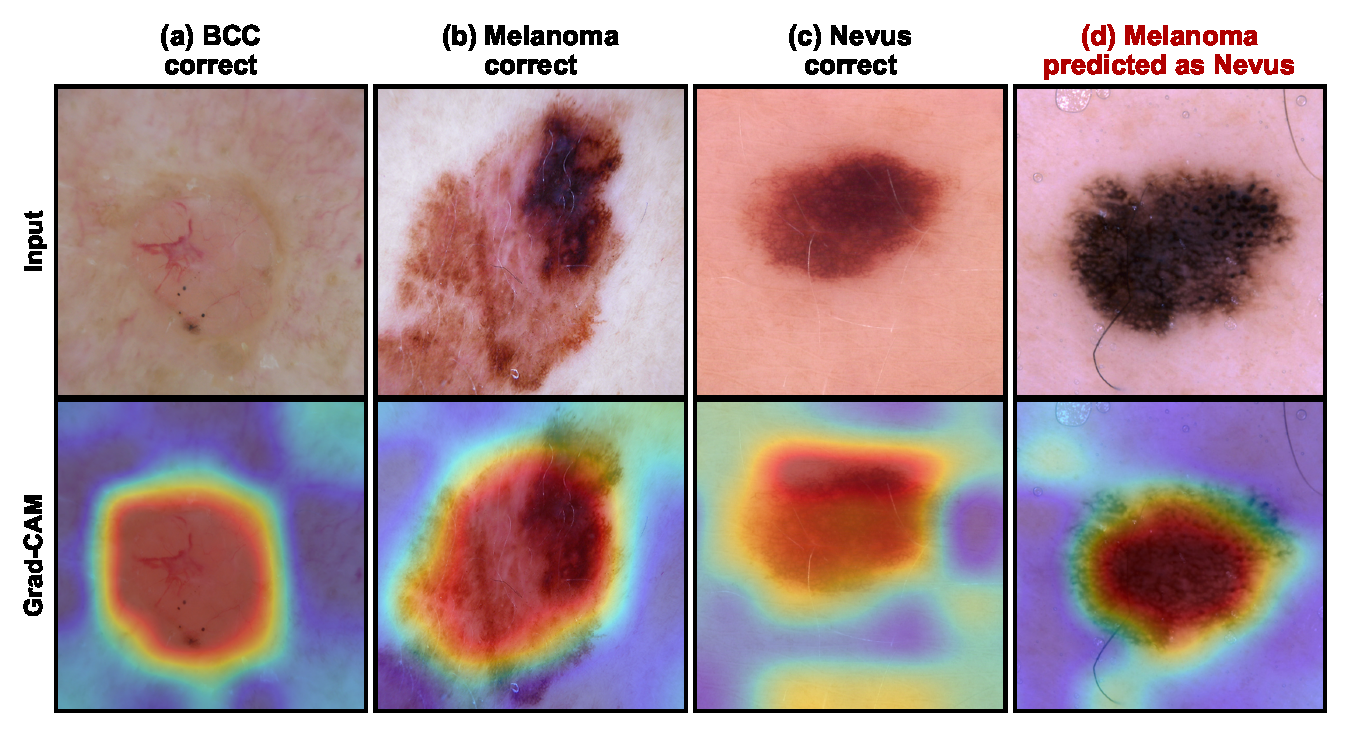
\includegraphics[width=0.78\textwidth]{gradcam_figure.pdf}\\[4pt]
\small\textbf{Grad-CAM heatmaps of MobileNetV2 (Fig.~5 of the revised manuscript): (a)--(c) correct BCC, Melanoma, and Nevus; (d) Melanoma predicted as Nevus.}
\end{center}

\textbf{Revised in the manuscript} (Sec.~6, Fig.~5 (p.~9)): ``\ldots\ \emph{In the failure case, the model also attends to the lesion but still predicts Nevus, which indicates that the error arises from how the lesion is interpreted rather than from attention to irrelevant regions.} \ldots''

\vspace{10pt}\noindent\rule{\textwidth}{0.4pt}\vspace{4pt}
\textbf{Comment 3.3:} \emph{Training settings should be reported.}

\textbf{Response:} We thank the reviewer for this suggestion. The training settings are reported in the methodology: input size ($224\times224$), normalization for each model, the augmentations used (rotation, zoom, translation), ImageNet and self-supervised pretraining, the classification heads, and 50 training epochs for both models, with the epoch-wise curves in Fig.~3. Owing to the ten-page limit, they are given in the text rather than in a separate table.

\textbf{Revised in the manuscript} (Sec.~3.3 (p.~4)): ``\ldots\ \emph{The verified MobileNetV2 training pipeline used rotation, zoom, and translation augmentation.} \ldots''

\vspace{10pt}\noindent\rule{\textwidth}{0.4pt}\vspace{4pt}
\textbf{Comment 3.4:} \emph{Fairness across skin tones should be discussed.}

\textbf{Response:} We thank the reviewer for raising this important point. ISIC 2019 does not provide Fitzpatrick skin-type labels and contains few images of darker skin, so a reliable subgroup analysis is not possible with this dataset, and colour-based skin-tone estimates from dermoscopic images are themselves unreliable. The manuscript therefore states this explicitly as a limitation and does not claim that performance generalizes across skin tones.

\textbf{Revised in the manuscript} (Sec.~5 (p.~8)): ``\ldots\ \emph{Apart from the McNemar test of the fusion audit, no confidence intervals, skin-tone fairness evaluation, or lesion-disjoint retrained test result are available in the present study.} \ldots''

\vspace{10pt}\noindent\rule{\textwidth}{0.4pt}\vspace{4pt}
\textbf{Comment 3.5:} \emph{Recent edge-oriented skin lesion classifiers should be cited.}

\textbf{Response:} We thank the reviewer for this suggestion. The revised manuscript now cites the efficient-model and compression literature on which the edge results build: MobileNet and MobileNetV2, integer-only quantization, post-training quantization, magnitude pruning, and transformer quantization. Because the edge claim rests on direct on-device measurements, the work is positioned against these methods rather than against systems evaluated on different devices, datasets, and class sets.

\textbf{Revised in the manuscript} (Sec.~4.5 (p.~7)): ``\ldots\ \emph{Layer-wise diagnostics identified extreme activation outliers in transformer Blocks 8--11, a known obstacle to post-training transformer quantization, with magnitudes up to approximately 494.72 compared with upper-percentile values near 1.3--2.7 in the corresponding diagnostic summaries.} \ldots''

\vspace{10pt}\noindent\rule{\textwidth}{0.4pt}\vspace{4pt}
\textbf{Comment 3.6:} \emph{Future work could include all ISIC classes.}

\textbf{Response:} We thank the reviewer for this suggestion. Future work now includes extending the study to all eight ISIC 2019 categories, together with lesion-disjoint retraining, quantization-aware training, and ViT-S distillation.

\textbf{Revised in the manuscript} (Sec.~7 (p.~9)): ``\ldots\ \emph{Extending the study to all eight ISIC 2019 categories, quantization-aware training, ViT-S distillation, out-of-distribution rejection, and imbalance-aware losses may improve the reliability of a future deployment-oriented system.} \ldots''


\vspace{12pt}
\section*{Editorial requirements}
\begin{itemize}
\item \textbf{Figures:} all figures were produced by the authors for this manuscript from their own experiments.
\item \textbf{References:} seven references were added (quantization, pruning, Grad-CAM, TensorFlow, transformer activation outliers), four previously uncited references are now cited, and the list is numbered in order of citation.
\end{itemize}

\medskip
Sincerely,\\
Darapureddi Chetan Kumar and Jinka Venkata Aravind

\end{document}
